% Basic stuff
\documentclass[a4paper,10pt]{article}
\usepackage[utf8]{inputenc}
\usepackage[nswissgerman]{babel}
\usepackage{scrextend}
\usepackage{lipsum}
\usepackage{gauss}
\usepackage{amssymb} % to import \leadsto

% 3 column landscape layout with fewer margins
\usepackage[landscape, left=0.75cm, top=1cm, right=0.75cm, bottom=1.5cm, footskip=15pt]{geometry}
\usepackage{flowfram}
\usepackage{floatrow}
\usepackage{amsmath}
\usepackage[inline]{enumitem}
\usepackage{pst-node}
\usepackage{auto-pst-pdf}
\usepackage{tikz}
\usepackage{tikz-cd} 
\usepackage{multicol}

\usetikzlibrary{calc,matrix}

\changefontsizes[9pt]{8pt}
\ffvadjustfalse
\setlength{\columnsep}{1cm}
\Ncolumn{3}
\DeclareMathOperator{\Tr}{Tr}
\DeclareMathOperator{\Sign}{sign}
\DeclareMathOperator{\Rank}{Rank}
\DeclareMathOperator{\Image}{Im}
\DeclareMathOperator{\Columnspace}{\mathcal{R}}
\DeclareMathOperator{\Nullspace}{\mathcal{N}}
\DeclareMathOperator{\Kernel}{Ker}
\DeclareMathOperator{\diag}{diag}
\DeclareMathOperator{\Span}{span}
\DeclareMathOperator{\Arg}{Arg}
\DeclareMathOperator{\Log}{Log}

\newcommand*{\hermconj}{\mathsf{H}}
\renewcommand{\arraystretch}{1.5} % Increases the row spacing

% define nice looking boxes
\usepackage[most]{tcolorbox}

% a base set, that is then customised
\tcbset {
  base/.style={
    boxrule=0mm,
    leftrule=1mm,
    left=1.75mm,
    arc=0mm, 
    fonttitle=\bfseries, 
    colbacktitle=black!10!white, 
    coltitle=black, 
    toptitle=0.75mm, 
    bottomtitle=0.25mm,
    title={#1}
  }
}

\newcommand{\middot}{~\textperiodcentered~}
\newlist{rowlist}{enumerate*}{1}
\setlist[rowlist]{label={\textbf{\roman*}\text{: }}, afterlabel={}, itemjoin=\middot}

\newlist{vaxioms}{enumerate*}{1}
\setlist[vaxioms]{label={\textbf{V\arabic*}\text{: }}, afterlabel={}, itemjoin=\middot}

\makeatletter
\renewcommand*\env@matrix[1][*\c@MaxMatrixCols c]{%
  \hskip -\arraycolsep
  \let\@ifnextchar\new@ifnextchar
  \array{#1}}
\makeatother

\newcommand\undermat[2]{%
  \makebox[0pt][l]{$\smash{\underbrace{\phantom{%
    \begin{matrix}#2\end{matrix}}}_{\text{$#1$}}}$}#2}

\newcommand\overmat[2]{%
  \makebox[0pt][l]{$\smash{\overbrace{\phantom{%
    \begin{matrix}#2\end{matrix}}}^{\text{$#1$}}}$}#2}

\definecolor{brandblue}{rgb}{0.34, 0.7, 1}
\newtcolorbox{mainbox}[1]{
  colframe=brandblue, 
  base={#1}
}

\newtcolorbox{subbox}[1]{
  colframe=black!20!white,
  base={#1}
}

% Mathematical typesetting & symbols
\usepackage{amsthm, mathtools, amssymb} 
\usepackage{marvosym, wasysym}
\allowdisplaybreaks

% Tables
\usepackage{tabularx, multirow}
\usepackage{booktabs}

% Make enumerations more compact
\usepackage{enumitem}
\setitemize{itemsep=0.5pt}
\setenumerate{itemsep=0.75pt}

% To include sketches & PDFs
\usepackage{graphicx}

% For hyperlinks
\usepackage{hyperref}
\hypersetup{
  colorlinks=true
}

% Metadata
\title{Cheatsheet Komplexe Analysis}
\author{Thomas Gassmann}
\date{Februar 2024}

% Math helper stuff
\def\limn{\lim_{n\to \infty}}
\def\limxo{\lim_{x\to 0}}
\def\limxi{\lim_{x\to\infty}}
\def\limxn{\lim_{x\to-\infty}}
\def\sumk{\sum_{k=1}^\infty}
\def\sumn{\sum_{n=0}^\infty}
\def\R{\mathbb{R}}
\def\C{\mathbb{C}}
\def\E{\mathbb{E}}
\def\K{\mathbb{K}}
\def\dx{\text{ d}x}
\def\dt{\text{ d}t}
\def\Re{\text{Re}}
\def\Im{\text{Im}}

\newcommand{\overbar}[1]{\mkern 1.5mu\overline{\mkern-1.5mu#1\mkern-1.5mu}\mkern 1.5mu}

\begin{document}


\begin{center}
    Lizenziert unter CC BY-SA 4.0. Für Urheber, Quellen und Lizenzinformationen, siehe:\\
    \href{https://github.com/thomasgassmann/eth-cheatsheets}{github.com/thomasgassmann/eth-cheatsheets}

    GITCOMMIT
\end{center}


Credits: \begin{rowlist}
    \item \href{https://github.com/XYQuadrat/eth-cheatsheets}{xyquadrat}
\end{rowlist}

\section{Vorwissen}
\subsection{Komplexe Zahlen}
\begin{mainbox}{Definition}
Ein Ausdruck der Form $z = a + ib$, wobei $i^2 = -1$. $a = \Re(z)$ ist der Realteil, $b = \Im(z)$ ist der Imaginärteil.
\end{mainbox}

Addition erfolgt komponentenweise, Multiplikation erfolgt unter Annahme des Binomialgesetzes und $i^2 = -1$ (i.e. $z w = (a c - b d) + i (a d + b  c)$). Für Division gilt $\frac{z}{w} = \frac{c + id}{a + ib} = \frac{z\overbar{w}}{w\overbar{w}} = \frac{(ca + bd) + i(ad - cb)}{a^2 + b^2}$.\\
Die Norm ist definiert als $|z| = \sqrt{\Re(z)^2 + \Im(z)^2} = \sqrt{z \cdot \overbar{z}}$. Für $z = x + iy$ ist $\overbar{z} = x - iy$ konjugiert-komplex.

\begin{subbox}{Multiplikation mit konjugierter Zahl}
$$z \overbar{z} = \Re(z)^2 + \Im(z)^2$$
\end{subbox}

Eine komplexe Zahl kann in Polarkoordinaten dargestellt werden. Es gilt $z = re^{i\phi} = r(\cos(\phi) + i\sin(\phi))$.
Radizieren: $\sqrt[n]{a} = z \iff a = z^n \iff |a| e^{i\alpha} = r^n e^{i\phi n}$ wobei $r = \sqrt[n]{|a|}$ und $\phi = \frac{\alpha + 2k\pi}{n}$.

\begin{mainbox}{Fundamentalsatz der Algebra}
  Sei $p(z) = a_n z^n + \cdots + a_0$ ein Polynom mit $a_n \neq 0$ und reellen oder komplexen Koeffizienten $a_i \in \mathbb{C}$. Dann existieren $w_1, \ldots, w_n \in \C$ mit:
  $$
    p(z) = a_n (z - w_1) (z - w_2) \ldots (z - w_n)
  $$
\end{mainbox}

Es gilt $\overbar{z \pm w} = \overbar{z} \pm \overbar{w}$, $\overbar{zw} = \overbar{z}\overbar{w}$, $\overbar{(\frac{z}{w})} = \frac{\overbar{z}}{\overbar{w}}$, $|\overbar{z}| = |z|$, $|z + w| \leq |z| + |w|$, $|zw| = |z| |w|$.

$$
\theta = \begin{cases}
  \arctan(\frac{y}{x}) \textbf{ if z on positive x-axis}\\
  \frac{\pi}{2} \textbf{ if }x=0, y > 0\\
  \pi + \arctan(\frac{y}{x}) \textbf{ if z on negative x-axis}\\
  \frac{3\pi}{2} \textbf{ if }x=0, y < 0
\end{cases}
$$

Das Argument $\arg(z)$ einer komplexen Zahl $z \neq 0$ ist als Winkelmass nur bis auf ganzzahlige Vielfache von $2\pi$ bestimmt. Um eine eindeutig bestimmte reelle Zahl zu bekommen können wir entscheiden, Winkel mit mit reellen Zahlen im Intervall $(-\pi,\pi]$ zu messen. Definitionsgemäss ist das die eindeutig bestimmte reelle Zahl
$$
\Arg(z) \in (-\pi, \pi]
$$
für die $z = r(\cos(\varphi) + i \sin(\varphi))$ mit $r = |z|$ und $\varphi = \Arg(z)$ gilt.

\begin{mainbox}{Komplexer Logarithmus}
  Sei $z \in C$. \textbf{Ein} Logarithmus von $z$ ist eine Zahl $w \in \C$ mit $\exp(w) = z$. Jede komplexe Zahl ausser $z = 0$ besitzt einen eindeutigen komplexen Logarithmus $w = s + it$ mit $t \in (-\pi, \pi]$. Alle anderen Logarithmen von $z$ sind durch $w + 2\pi ik$ für $\k \in \mathbb{Z}$ gegeben.

  Für $z \neq 0$ ist der Hauptwert des Logarithmus von $z$ definiert durch:
  $$
    \Log(z) := \log(|z|) + i \Arg(z)
  $$
\end{mainbox}

Sei \(z\) eine komplexe Zahl und \(n\geq2\) eine ganze Zahl. Eine \(n\)-te Wurzel von \(z\) ist eine komplexe Zahl \(w\), die \(w^n=z\) erfüllt.

\subsection{Mengen}

\begin{subbox}{Offene Kreisscheibe}
  Sei $z_0\in\mathbb{C}$ und sei $r$ eine positive reelle Zahl. Die offene Kreisscheibe mit Zentrum $z_0$ und Radius $r$ ist die Teilmenge
  $$
  B(z_0, r) := \{ z \in \mathbb{C} : \, |z-z_0| < r \}
  $$
  von $\mathbb{C}$.
\end{subbox}

Eine Teilmenge $U \subseteq \C$ heisst offen, wenn zu jedem $z \in U$ ein Radius $\epsilon>0$ existiert, so dass $B(z,\epsilon) \subseteq U$ gilt.

\subsection{Folgen und Reihen}

\begin{mainbox}{Konvergenz}
  Sei \(z_1,z_2,z_3,\ldots\) eine Folge komplexer Zahlen. Wir sagen \(z \in \mathbb{C}\) sei der Grenzwert dieser Folge, und dass die Folge gegen \(z\) konvergiert, falls es für jede noch so kleine positive reelle Zahl \(\epsilon>0\) eine ganze Zahl \(N>0\) gibt, so dass \[|z-z_n|<\epsilon \text{ für alle } n\geq N \] gilt. In diesem Fall schreiben wir \(\displaystyle\lim_{n\to\infty}z_n=z\).
\end{mainbox}

\begin{subbox}{Leibnizkriterium}
Wenn $a_n \ge 0, \ \forall n \ge 1$ monoton fallend (ab gewissen $n_0$) ist und $\limn a_n = 0$ gilt, dann konvergiert $S = \sumk (-1)^{k+1} a_k$ und $a_1 - a_2 \le S \le a_1$.
\end{subbox}

\begin{mainbox}{Quotientenkriterium}
Sei $(a_n)$ eine Folge mit $a_n \ne 0, \forall n \ge 1$. \\ Falls $\limn \sup \frac{|a_{n+1}|}{|a_n|} < 1 \implies \sum_{n=1}^\infty a_n$ konvergiert absolut. \\Falls $\limn \inf \frac{|a_{n+1}|}{|a_n|} > 1 \implies \sum_{n=1}^\infty a_n$ divergiert.  
\end{mainbox}

\begin{mainbox}{Wurzelkriterium}
Sei $(a_n)$ eine Folge mit $a_n \ne 0, \forall n \ge 1$. Sei $q = \limn \sup \sqrt[n]{|a_n|}$. 
\begin{itemize}
 \item $q < 1 \implies \sum_{n=1}^\infty a_n$ konvergiert absolut.
 \item $q = 1 \implies$ keine Aussage.
 \item $q > 1 \implies \sum_{n=1}^\infty a_n$ und $\sum_{n=1}^\infty |a_n|$ divergieren.
\end{itemize}
\end{mainbox}


\subsection{Potenzreihen}
\begin{subbox}{Definition Potenzreihe}
 Potenzreihen sind Reihen der Form $\sum_{n=0}^\infty c_n x^n$. Eine Potenzreihe mit Entwicklungspunkt $x_0$ wird als $\sum_{n=0}^\infty c_n(x-x_0)^n$ definiert.
\end{subbox}

\begin{mainbox}{Konvergenzradius}
 Der Konvergenzradius einer Potenzreihe $\sumn a_n x^n$ um einen Entwicklungspunkt $x_0$ ist die grösste Zahl $r$, so dass die Potenzreihe für alle $x$ mit $|x - x_0| < r$ konvergiert. Falls die Reihe für alle $x$ konvergiert, ist der Konvergenzradius $r$ unendlich. Sonst:
 $$r = \begin{cases}
    +\infty & \text{ falls } \limn\sup \sqrt[n]{|a_n|} = 0\\
    \frac{1}{\limn\sup \sqrt[n]{|a_n|}} & \text{ falls }  \limn\sup \sqrt[n]{|a_n|} > 0
 \end{cases} $$
 Alternativ, falls existiert, kann $r = \limn \left| \frac{a_n}{a_{n+1}} \right|$ verwendet werden (weniger starke Aussage).\\
 Dies folgt aus dem Wurzelkriterium für $a_n := c_n z^n$. Also wollen wir $\sqrt[n]{|a_n|} \overset{!}{<} 1$ und können dann nach $|z|$ umformen. Hilfreich, wenn nicht exakt $z^n$-Format vorhanden ist.
\end{mainbox}
Die Potenzreihe $\sum_{k=0}^\infty c_n x^n$ konvergiert absolut und gleichmässig für alle $|x| < r$ und divergiert für alle $|x| > r$. Der Fall $|x| = r$ ist unklar und muss geprüft werden.

\subsubsection{Potenzreihen}
\begin{align*}
\exp(x) &= \sumn \frac{x^n}{n!} = 1 + x + \frac{x^2}{2!} + \frac{x^3}{3!} + \cdots & r &= \infty \\
\sin(x) &= \sumn (-1)^n \frac{x^{2n + 1}}{(2n + 1)!} = x - \frac{x^3}{3!} + \frac{x^5}{5!} - \cdots & r &= \infty \\
\cos(x) &= \sumn (-1)^n \frac{x^{2n}}{(2n)!} = 1 - \frac{x^2}{2!} + \frac{x^4}{4!} - \cdots & r &= \infty \\
\ln(x + 1) &= \sumk (-1)^{k+1} \frac{x^k}{k} = x - \frac{x^2}{2} + \frac{x^3}{3} - \cdots & r &= 1 \\
\sinh(x) &= \sumn \frac{x^{2n+1}}{(2n+1)!} & r &= \infty \\
\cosh(x) &= \sumn \frac{x^{2n}}{(2n)!} & r &= \infty \\
\arctan(x) &= \sumn (-1)^n \frac{x^{2n+1}}{2n+1} & r &= 1 \\
e^{-x} &= \sumn (-1)^n \cdot \frac{x^n}{n!} & r &= \infty \\
\end{align*}


\subsubsection{Wichtige Reihen}
\begin{align*}
 \sum_{i=1}^n i &= \frac{n(n+1)}{2} \\
 \sum_{i=1}^n i^2 &= \frac{1}{6}n(n+1)(2n+1) \\
 \sum_{i=1}^n i^3 &= \frac{1}{4}n^2(n+1)^2 \\
 \sum_{i=1}^\infty \frac{1}{i^2} &= \frac{\pi^2}{6} \\
 \sum_{n=1}^\infty \frac{1}{n(n+1)} &= 1
\end{align*}

\subsubsection{Cauchy-Produkt}
$\sumk b_k$ ist eine \textbf{lineare Anordnung} der Doppelreihe $\Sigma_{i,j \geq 0} a_{i,j}$, falls es eine Bijektion $\sigma : \mathbb{N} \rightarrow \mathbb{N} \times \mathbb{N}$ gibt, mit $b_k = a_{\sigma(k)}$.\\

\begin{subbox}{Konvergenz Doppelreihe}
  Wenn es $B \geq 0$ gibt, so dass $\Sigma_{i=0}^m \Sigma_{j=0}^m |a_{ij}| \leq B$ $\forall m \geq 0$, dann konvergieren $S_i := \Sigma_{j=0}^\infty a_{ij}$ $\forall i \geq 0$ und $U_j := \Sigma_{i=0}^\infty a_{ij}$ $\forall j \geq 0$ sowie $\Sigma_{i=0}^\infty S_i$, $\Sigma_{j=0}^\infty U_j$ und es gilt $\Sigma_{i=0}^\infty S_i = \Sigma_{j=0}^\infty U_j$. Jede lineare Anordnung einer Doppelreihe konvergiert dann absolut mit demselben Grenzwert.
\end{subbox}

\begin{subbox}{Tauschbarkeit Summation / Limes}
  Sei $f_n : \mathbb{N} \rightarrow \mathbb{R}$ eine Folge. Wenn $f(j) := \limn f_n(j)$ $\forall j \in \mathbb{N}$ existiert und $|f_n(j)| \leq g(j)$ für eine Funktion $g: \mathbb{N} \rightarrow \mathbb [0, \infty[$ und falls $\sum_{j=0}^\infty g(j)$ konvergiert, dann folgt $\sum_{j=0}^\infty f(j) = \limn \sum_{j=0}^\infty f_n(j)$.
\end{subbox}

\begin{mainbox}{Cauchy-Produkt}
  Das Cauchy-Produkt von zwei Reihen $\sum_{i = 0}^\infty a_i$ und $\sum_{j = 0}^\infty b_j$ ist definiert als
  $$\sum_{n=0}^\infty \sum_{j=0}^n (a_{n-j} \cdot b_j) = a_0b_0 + (a_0b_1 + a_1b_0) + \ldots$$ Es konvergiert, falls beide Reihen absolut konvergieren. Dann gilt:\\
  $$\sum_{n=0}^\infty \sum_{j=0}^n (a_{n-j} \cdot b_j) = (\sum_{i=0}^\infty a_i) (\sum_{j=0}^\infty b_j)$$
\end{mainbox}


\subsubsection{Strategie - Konvergenz von Reihen}
\begin{enumerate}
 \item Ist Reihe ein bekannter Typ? (Teleskopieren, Geometrische/Harmonische Reihe, Zetafunktion, ...){
  \begin{itemize}
    \item Beim Teleskopieren einer Teleskopreihe $S_n = \sum_{k=0}^n a_k = \sum_{k=0}^n (a_k - a_{k+1}) = a_0 - a_{n+1}$ kann man den Limes von der rechten Seite nehmen.
  \end{itemize}
 }
 \item Ist $\limn a_n = 0$? Wenn nein, divergent.
 \item Leibnizkriterium anwenden, falls alternierend
 \item Quotientenkriterium für Exponentialfunktionen oder Fakultäten
 \item Wurzelkriterium
 \item Vergleichssatz anwenden, Vergleichsreihen suchen, konvergente Majorante oder divergente Minorante
 \item Integral-Test anwenden (Reihe zu Integral)
\end{enumerate}


\subsection{Polynome}

Bei Polynomen mit reellen Nullstellen treten die Nullstellen als komplex-konjugiertes Paar auf. Für Grad 2, verwende $z = \frac{-b \pm \sqrt{b^2 - 4ac}}{2a}$ um ein Polynom $p(z) = 0$ zu lösen. Für $a z^n + c = 0$, verwende $z = \sqrt[n]{-\frac{c}{a}}$.

Bei einem Polynom über $\mathbb{C}$ mit ungeradem Grad gibt es mindestens eine reelle Nullstelle.

\section{Komplexwertige Funktionen}

\subsection{Ableitung komplexwertiger Funktionen}

\begin{subbox}{Stetigkeit}
  Sei \(U\subseteq\mathbb{C}\) eine offene Teilmenge. Eine Funktion \(f\colon U\to\mathbb{C}\) heisst stetig im Punkt \(z_0\in U\), falls es für jedes \(\epsilon>0\) ein \(\delta >0\) gibt, so dass für alle \(z\in U\) die Implikation \[|z-z_0|<\delta ~\implies ~ |f(z)-f(z_0)|< \epsilon\] gilt. Wir sagen \(f\) sei stetig auf \(U\), falls \(f\) stetig in jedem Punkt von \(U\) ist.

  $f$ ist stetig in $z_0$ genau dann wenn $\lim_{z \to z_0} f(z) = f(z_0)$.
\end{subbox}

\begin{subbox}{Grenzwert}
  Sei \(U\subseteq\mathbb{C}\) eine offene Teilmenge, \(z_0\in U\) und \(f\colon U\smallsetminus\{z_0\}\to\mathbb{C}\) eine Funktion. Eine komplexe Zahl \(a\) nennt man den Grenzwert von \(f\) in \(z_0\) und schreibt
  $$
  \lim_{z\to z_0}f(z)=a
  $$
  
  falls es für jedes \(\epsilon>0\) ein \(\delta>0\) gibt, so dass für alle \(z\in U\), \(z\neq z_0\), die Implikation 
  $$
  0<|z-z_0|<\delta ~\implies ~ |f(z)-a|<\epsilon
  $$ gilt. Der Grenzwert existiert nur falls er unabhängig von der Richtung ist.
\end{subbox}

\begin{subbox}{Komplexe Differenzierbarkeit}
  Sei \(U \subseteq \mathbb{C}\) offen und \(f \colon U \to \mathbb{C}\) eine Funktion. Wir sagen, dass \(f\) $\C$-differenzierbar in \(z_0 \in U\) ist, falls:
  $$
  f'(z_0) = \frac{df}{dz}(z_0) = \lim_{z \to z_0} \dfrac{f(z)-f(z_0)}{z-z_0}
  $$
  existiert. Differenzierbarkeit impliziert Stetigkeit.
\end{subbox}

\begin{itemize}
  \item Linearität der Ableitung
  $$(\alpha \cdot f(x) + g(x))' = \alpha \cdot f'(x) + g'(x)$$
  \item Produktregel
  $$(f(x) \cdot g(x))' = f'(x) \cdot g(x) + f(x) \cdot g'(x)$$
  \item Quotientenregel ($g(x) \neq 0$)
  $$\left(\frac{f(x)}{g(x)}\right)' = \frac{f'(x) \cdot g(x) - f(x) \cdot g'(x)}{g(x)^2}$$
  \item Kettenregel
  $$(f(g(x)))' = g'(x) \cdot f'(g(x))$$
  \item Potenzregel
  $$(c \cdot x^a)' = c \cdot a \cdot x^{a - 1}$$
  \item{
    Inverse (bijektiv)
    $$
    (f^{-1})'(y_0) = \frac{1}{f'(x_0)} = \frac{1}{f'(f^{-1}(y_0))}
    $$
  }
\end{itemize}

\begin{mainbox}{Holomorphische Funktionen}
  Eine Funktion $f: U \to \C$ heisst \textbf{holomorph auf $U$} falls sie auf der ganzen Menge $U$ $\C$-differenzierbar ist. Die Funktion heisst \textbf{holomorph in $z_0 \in U$} falls in einer offenen Menge um $z_0$ holomorph ist.
\end{mainbox}

Falls eine Funktion $\overbar{z}$ enthält, so ist sie nie holomorph.

\subsection{Cauchy-Riemann Gleichungen}


\section{Taylor- und Laurentreihen}

\section{Fourier-Analysis}

\section{Laplace-Transformation}

\section{Tabellen und Listen}

\subsection{Ungleichungen}

\begin{itemize}
  \item Dreiecksungleichung: $|a + b| \leq |a| + |b|$
  \item umgekehrte Dreiecksungleichung: $||a| - |b|| \leq |a \pm b| \leq |a| + |b|$ für alle $a,b \in \R$
  \item $(1+x)^n \geq 1+ n\cdot x$ \, $\forall n\in \mathbb{N}, x > -1$
  \item $e^x \geq 1 + x$ \, $\forall x\in \mathbb{R}$
  \item $2|xy| \leq \epsilon x^2 + \frac{1}{\epsilon} y^2$ für $\forall \epsilon > 0$ und $\forall x,y \in \mathbb{R}$
  \item $|\langle x,y \rangle| \leq ||x|| \cdot ||y||$ für $\forall x,y, \in \mathbb{R}^n$
  \item $\sqrt[n]{x_1 x_2 \cdots x_n} \leq \frac{x_1 + x_2 + \cdots + x_n}{n}$
  \item $\left| \int_A f(x) \mathop{dx}\right| \le \int_A \left|f(x)\right| \mathop{dx}$
\end{itemize}

\subsection{Trigonometrie}

\subsubsection{Doppelwinkel}
\begin{itemize}
 \item $\sin(2\alpha) = 2 \sin(\alpha) \cos(\alpha)$
 \item $\cos(2\alpha) = \cos^2(\alpha) - \sin^2(\alpha) = 1 - 2 \sin^2(\alpha)$
 \item $\tan(2\alpha) = \frac{2\tan(\alpha)}{1 - \tan^2(\alpha)}$
\end{itemize}

\subsubsection{Addition}
\begin{itemize}
 \item $\sin(\alpha + \beta) = \sin(\alpha) \cos(\beta) + \cos(\alpha) \sin(\beta)$
 \item $\cos(\alpha + \beta) = \cos(\alpha) \cos(\beta) - \sin(\alpha) \sin(\beta)$
 \item $\tan(\alpha + \beta) = \frac{\tan(\alpha) + \tan(\beta)}{1 - \tan(\alpha) \tan(\beta)}$
\end{itemize}

\subsubsection{Subtraktion}
\begin{itemize}
 \item $\sin(\alpha - \beta) = \sin(\alpha) \cos(\beta) - \cos(\alpha)\sin(\beta)$
 \item $\cos(\alpha - \beta) = \cos(\alpha) \cos(\beta) + \sin(\alpha)\sin(\beta)$
 \item $\tan(\alpha - \beta) = \frac{\tan(\alpha) - \tan(\beta)}{1+\tan(\alpha) \tan(\beta)}$
\end{itemize}

\subsubsection{Multiplikation}
\begin{itemize}
 \item $\sin(\alpha) \sin(\beta) = -\frac{\cos(\alpha + \beta) - \cos(\alpha - \beta)}{2}$
 \item $\cos(\alpha) \cos(\beta) =  \frac{\cos(\alpha + \beta) + \cos(\alpha - \beta)}{2}$
 \item $\sin(\alpha) \cos(\beta) =  \frac{\sin(\alpha + \beta) + \sin(\alpha - \beta)}{2}$
\end{itemize}

\subsubsection{Potenzen}
\begin{itemize}
 \item $\sin^2(\alpha) = \frac{1}{2}(1-\cos(2\alpha))$
 \item $\cos^2(\alpha) = \frac{1}{2}(1+\cos(2\alpha))$
 \item $\tan^2(\alpha) = \frac{1-\cos(2\alpha)}{1+\cos(2\alpha)}$
 \item $\sin^3(\alpha) = \frac{3}{4} \sin(\alpha) - \frac{1}{4} \sin(3 \alpha)$
 \item $\cos^3(\alpha) = \frac{3}{4} \cos(\alpha) + \frac{1}{4} \cos(3 \alpha)$
\end{itemize}

\subsubsection{Hyperbolische Trigonometrische Funktionen}
\begin{itemize}
  \item $\cosh^2(\alpha) - \sinh^2(\alpha) = 1$
  \item $\sinh(x) = \frac{e^x - e^{-x}}{2}$ und $\cosh(x) = \frac{e^x + e^{-x}}{2}$
  \item $\sin(ix) = i \sinh(x)$
 \end{itemize}

\subsubsection{Diverse}

\begin{itemize}
 \item $\sin^2(\alpha) + \cos^2(\alpha) = 1$
 \item $\sin(z) = \frac{e^{iz} - e^{-iz}}{2i}$ und $\cos(z) = \frac{e^{iz} + e^{-iz}}{2}$
 \item $\cos(x)^n = \frac{1}{2^n} \sum_{k=0}^n {n \choose k} \cos((2k - n)x)$
 \item $\cos(x) = \Re(e^{ix})$, $\sin(x) = \Im(e^{ix})$
\end{itemize}


\begin{center}
  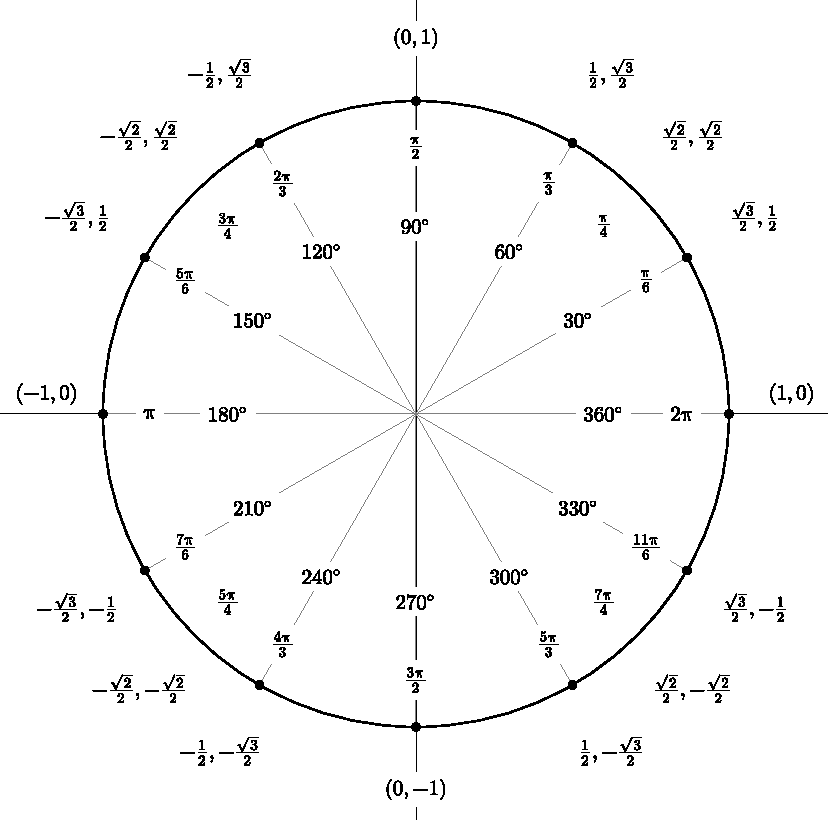
\includegraphics[width= \linewidth]{include_degrees_circle.pdf}
\end{center}

\begin{mainbox}{Trigonometrische Funktionen}
  \begin{center} 
    \begin{tabular}{c|cccccc}
      deg & 0° & 30° & 45° & 60° & 90° & 180° \\
      \midrule
      rad & 0 & $\frac{\pi}{6}$ & $\frac{\pi}{4}$ & $\frac{\pi}{3}$ & $\frac{\pi}{2}$ & $\pi$ \\
      cos & 1 & $\frac{\sqrt{3}}{2}$ & $\frac{\sqrt{2}}{2}$ & $\frac{1}{2}$ & 0 & -1 \\
      sin & 0 & $\frac{1}{2}$ & $\frac{\sqrt{2}}{2}$ & $\frac{\sqrt{3}}{2}$ & 1 & 0 \\
      tan & 0 & $\frac{1}{\sqrt{3}}$ & 1 & $\sqrt{3}$ & $+\infty$ & 0 \\
    \end{tabular}
  \end{center}
\end{mainbox}

\subsubsection{Trigonometrische Identitäten}
\begin{center}
 \begin{tabularx}{\linewidth}{>{\centering\arraybackslash}X>{\centering\arraybackslash}X}
  \toprule
  $\sin(\arccos (x))$ & $\sqrt{1-x^2}$\\
  $\cos(\arcsin(x))$ & $\sqrt{1-x^2}$\\
  $\sin(\arctan(x))$ & $\frac{x}{\sqrt{1+x^2}}$\\
  $\cos(\arctan(x))$ & $\frac{1}{\sqrt{1+x^2}}$\\
  $\tan(\arcsin(x))$ & $\frac{x}{\sqrt{1-x^2}}$\\
  $\tan(\arccos(x))$ & $\frac{\sqrt{1-x^2}}{x}$\\
  \bottomrule
 \end{tabularx}
\end{center}

\subsection{Rekursive Integrale}

$J_n = \int \frac{1}{(1 + x^2)^n} \dx$, dann $J_{n+1} = \frac{x}{2n(1 + x^2)^n} + (\frac{2n - 1}{2n})J_n$ mit $J_1 = \arctan(x)$.

\subsection{Binomischer Lehrsatz}

$$(x+y)^n = \sum_{k=0}^n {n \choose k} x^{n-k} y^k$$

\subsection{Uneigentliche Integrale}
$$\int_1^\infty \frac{1}{x^\alpha} \dx = \begin{cases}
  \text{divergiert, } & \alpha \leq 1\\
  \frac{1}{\alpha - 1} & \alpha > 1
\end{cases}$$
$$\int_0^1 \frac{1}{x^\alpha} \dx = \begin{cases}
  \text{divergiert, } & \alpha \geq 1\\
  \frac{1}{1- \alpha} & \alpha < 1
\end{cases}$$
$$\int_0^\infty e^{-x} \dx = 1$$
$$\int_0^\infty e^{-x}x^{s-1} \dx = \begin{cases}
  \text{divergiert, } & s \leq 0\\
  (s-1)! & s > 0
\end{cases}$$
$$\int_0^\infty \sin(x^2) \dx = \sqrt{\frac{\pi}{8}}$$

\subsection{Gerade und ungerade Funktionen}
\begin{itemize}
  \item Die Verknüpfung von ungeraden Funktionen ist ungerade. 
  \item Sei $g$ gerade und $f$ beliebig. $f \circ g$ ist gerade.
  \item Sei $f$ gerade und $g$ ungerade. $g \circ f$ und $f \circ g$ sind gerade.
  \item Produkt einer geraden und einer ungeraden Funktion ist ungerade.
  \item Produkt zweier ungerader Funktionen ist gerade.
  \item Produkt zweier gerader Funktionen ist gerade.
  \item Für $f: [-a, a] \to \mathbb{R}$ stetig und ungerade, d.h. $f(-x) = -f(x)$ gilt $\int_{-a}^a f(x) \dx = 0$.
\end{itemize}


\subsection{Weitere Tabellen}

\subsubsection{$n$-te Ableitungen}
\begin{center}
  \begin{tabularx}{\linewidth}{>{\centering\arraybackslash}X>{\centering\arraybackslash}X}
  \toprule
  $\mathbf{f(x)}$ & $\mathbf{f^{(n)}(x)}$ \\
  \midrule
  $\sin(x)$ & $\sin(\frac{n\pi}{2} + x)$\\
  $f + g$ & $f^{(n)} + g^{(n)}$\\
  $f \cdot g$ & $\sum\limits_{k=0}^{n}\binom{n}{k}f^{(k)}g^{(n-k)}$\\
  \bottomrule
  \end{tabularx}
\end{center}

\subsubsection{Ableitungen (I)}
\begin{center}
  \begin{tabularx}{\linewidth}{c>{\centering\arraybackslash}Xc}
  \toprule
  $\mathbf{F(x)}$ & $\mathbf{f(x)}$ & $\mathbf{f'(x)}$ \\
  \midrule
  $\frac{x^{-a+1}}{-a+1}$ & $\frac{1}{x^a}$ & $\frac{a}{x^{a+1}}$ \\
  $\frac{x^{a+1}}{a+1}$ & $x^a \ (a \ne -1)$ & $a \cdot x^{a-1}$ \\
  $\frac{1}{k \ln(a)}a^{kx}$ & $a^{kx}$ & $ka^{kx} \ln(a)$ \\
  $\ln |x|$ & $\frac{1}{x}$ & $-\frac{1}{x^2}$ \\
  $\frac{2}{3}x^{3/2}$ & $\sqrt{x}$ & $\frac{1}{2\sqrt{x}}$\\
  $-\cos(x)$ & $\sin(x)$ & $\cos(x)$ \\
  $\sin(x)$ & $\cos(x)$ & $-\sin(x)$ \\
  $\frac{1}{2}(x-\frac{1}{2}\sin(2x))$ & $\sin^2(x)$ & $2 \sin(x)\cos(x)$ \\
  $\frac{1}{2}(x + \frac{1}{2}\sin(2x))$ & $\cos^2(x)$ & $-2\sin(x)\cos(x)$ \\
  $-\ln|\cos(x)|$ & $\tan(x)$ & $\frac{1}{\cos^2(x)} = 1 + \tan^2(x)$  \\
  $\cosh(x)$ & $\sinh(x)$ & $\cosh(x)$ \\
  $\log(\cosh(x))$ & $\tanh(x)$ & $\frac{1}{\cosh^2(x)} = 1 - \tanh^2(x)$ \\
  $\ln | \sin(x)|$ & $\cot(x)$ & $-\frac{1}{\sin^2(x)}$ \\
  $\frac{1}{c} \cdot e^{cx}$ & $e^{cx}$ & $c \cdot e^{cx}$ \\
  $x(\ln |x| - 1)$ & $\ln |x|$ & $\frac{1}{x}$ \\
  $\frac{1}{2}(\ln(x))^2$ & $\frac{\ln(x)}{x}$ & $\frac{1 - \ln(x)}{x^2}$ \\
  $\frac{x}{\ln(a)} (\ln|x| -1)$ & $\log_a |x|$ & $\frac{1}{\ln(a)x}$ \\
  $\frac{1}{2}(\cosh(x)\sinh(x)+1)$ & $\cosh(x)^2$ & $2\sinh(x)\cosh(x)$\\
  $\frac{1}{2}(\sinh(x)\cosh(x) + x)$ & $\sinh(x)^2$ & $2\sinh(x)\cosh(x)$\\
  \bottomrule
  \end{tabularx}
\end{center}

\subsubsection{Weitere Ableitungen}
\begin{center}
  \begin{tabularx}{\linewidth}{>{\centering\arraybackslash}X>{\centering\arraybackslash}X}
  \toprule
  $\mathbf{F(x)}$ & $\mathbf{f(x)}$ \\
  \midrule
  $\arcsin(x)$ & $\frac{1}{\sqrt{1 - x^2}}$ \\
  $\arccos(x)$ & $\frac{-1}{\sqrt{1 - x^2}}$ \\
  $\arctan(x)$ & $\frac{1}{1 + x^2}$ \\ 
  $\text{arsinh}(x)$ & $\frac{1}{\sqrt{1 + x^2}}$ \\
  $\text{arcosh}(x)$ & $\frac{1}{\sqrt{x^2 - 1}}$ \\
  $\text{artanh}(x)$ & $\frac{1}{1 - x^2}$ \\
  $\text{arccot}(x)$ & $-\frac{1}{1 + x^2}$ \\
  $x^x \ (x > 0)$ & $x^x \cdot (1 + \ln x)$ \\
  $\cosh(x)$ & $\sinh(x)$ \\
  $\sinh(x)$ & $\cosh(x)$ \\
  \bottomrule
  \end{tabularx}
\end{center}

\subsubsection{Grenzwerte}
\begin{center}
  \begin{tabularx}{\linewidth}{XX}
    \toprule
    $\limxi \frac{1}{x} = 0$ & $\limxi 1 + \frac{1}{x} = 1$ \\
    $\limxi e^x = \infty$ & $\limxn e^x = 0$ \\
    $\limxi e^{-x} = 0$ & $\limxn e^{-x} = \infty$ \\
    $\limxi \frac{e^x}{x^m} = \infty$ & $\limxn xe^x = 0$ \\
    $\limxi \ln(x) = \infty$ & $\limxo \ln(x) = -\infty$ \\
    $\limxi (1+x)^{\frac{1}{x}} = 1$ & $\limxo (1+x)^{\frac{1}{x}} = e$ \\
    $\limxi (1+\frac{1}{x})^b = 1$ & $\limxi n^{\frac{1}{n}} = 1$ \\
    $\lim_{x\to\pm\infty} (1 + \frac{1}{x})^x = e$ & $\limxi (1-\frac{1}{x})^x = \frac{1}{e}$ \\
    $\lim_{x\to\pm\infty} (1 + \frac{k}{x})^{mx} = e^{km}$ & $\limxi (\frac{x}{x+k})^x = e^{-k}$ \\
    $\limxo \frac{a^x -1}{x} = \ln(a), \newline \forall a > 0$ &
    $\limxi x^a q^x = 0, \newline \forall 0 \le q < 1$ \\
  \end{tabularx}
  \begin{tabularx}{\linewidth}{XX}
    $\limxo \frac{\sin x}{x} = 1$ & $\limxo \frac{\sin kx}{x} = k$\\
    $\limxo \frac{1}{\cos x} = 1$ & $\limxo \frac{\cos x -1}{x} = 0$ \\
    $\limxo x \sin(\frac{1}{x}) = 0$ & $\limxo x \log x = 0$\\
    $\limxo \frac{1 - \cos x}{x^2} = \frac{1}{2}$ & $\limxo \frac{e^x-1}{x} = 1$ \\
    $\limxo \frac{x}{\arctan x} = 1$ & $\limxi \arctan x = \frac{\pi}{2}$ \\
    $\limxo \frac{e^{ax}-1}{x} = a$ & $\limxo \frac{\ln(x+1)}{x} = 1$ \\
    $\lim_{x\to 1} \frac{\ln(x)}{x-1} = 1$ & $\limxi \sqrt{x^2 + c} - x = 0$ \\
    $\limxi \sqrt[x]{x} = 1$ & $\limxi x(\sqrt[x]{n} - 1) = \ln(n)$ \\
    \bottomrule
  \end{tabularx}
\end{center}

\subsubsection{Weitere Integrale}
\begin{center}
  \begin{tabularx}{\linewidth}{>{\centering\arraybackslash}X>{\centering\arraybackslash}X}
   \toprule
   $\mathbf{f(x)}$ & $\mathbf{F(x)}$ \\
   \midrule
   $\int f'(x) f(x) \dx$ & $\frac{1}{2}(f(x))^2$ \\
   $\int \frac{f'(x)}{f(x)} \dx$ & $\ln|f(x)|$ \\
   $\int_{-\infty}^\infty e^{-x^2} \dx$ & $\sqrt{\pi}$ \\
   $\int (ax+b)^n \dx$ & $\frac{1}{a(n+1)}(ax+b)^{n+1}$ \\
   $\int x(ax+b)^n \dx$ & $\frac{(ax+b)^{n+2}}{(n+2)a^2} - \frac{b(ax+b)^{n+1}}{(n+1)a^2}$ \\
   $\int (ax^p+b)^n x^{p-1} \dx$ & $\frac{(ax^p+b)^{n+1}}{ap(n+1)}$ \\
   $\int (ax^p + b)^{-1} x^{p-1} \dx$ & $\frac{1}{ap} \ln |ax^p + b|$ \\
   $\int \frac{ax+b}{cx+d} \dx$ & $\frac{ax}{c} - \frac{ad-bc}{c^2} \ln |cx +d|$ \\
   $\int \frac{1}{x^2+a^2} \dx$ & $\frac{1}{a} \arctan \frac{x}{a}$ \\
   $\int \frac{1}{x^2 - a^2} \dx$ & $\frac{1}{2a} \ln\left| \frac{x-a}{x+a} \right|$ \\
   $\int \sqrt{a^2 - x^2} \dx $ & $\frac{a^2}{2} \arcsin(\frac{x}{a}) + \frac{x}{2} \sqrt{a^2 - x^2}$ \\
   \bottomrule
  \end{tabularx} 
 \end{center}

 \subsubsection{Trigonometrische Integrale}

 \begin{center}
  \begin{tabularx}{\linewidth}{>{\centering\arraybackslash}X>{\centering\arraybackslash}X}
   \toprule
   $\mathbf{f(x)}$ & $\mathbf{F(x)}$ \\
   \midrule
   $\int \csc(x) \dx $ & $\ln|\csc(x) + \cot(x)|$ \\
   $\int \sec(x) \dx $ & $\ln|\sec(x) + \tan(x)|$ \\
   $\int \cot(x) \dx $ & $\ln|\sin(x)|$ \\
   $\int x \sin(ax) \dx$ & $-\frac{1}{a} x \cos(ax) + \frac{1}{a^2} \sin(ax)$ \\
   \bottomrule
  \end{tabularx} 
 \end{center}

\subsubsection{Fourier-Transformationen}

\subsubsection{Laplace-Transformationen}

\begin{center}
  \begin{tabularx}{\linewidth}{c>{\centering\arraybackslash}Xc}
  \toprule
  $f(t)$ & $\mathcal{L}[f(t)](s)$ \\
  \midrule
  1 & $\frac{1}{s}, \; \Re(s) >  0$ \\
  $t^n$ & $\frac{n!}{s^{n+1}}, \; \Re(s) >  0$ \\
  $\sin(at)$ & $\frac{a}{s^2 + a^2}, \; \Re(s) >  0$ \\
  $\cos(at)$ & $\frac{s}{s^2 + a^2}, \; \Re(s) >  0$ \\
  $e^{at}$ & $\frac{1}{s-a}, \; \Re(s) >  a$ \\
  $e^{at} \sin(bt)$ & $\frac{b}{(s-a)^2 + b^2}, \; \Re(s) >  a$ \\
  $e^{at} \cos(bt)$ & $\frac{s-a}{(s-a)^2 + b^2}, \; \Re(s) >  a$ \\
  $t^n e^{at}$ & $\frac{n!}{(s-a)^{n+1}}, \; \Re(s) >  a$ \\
  $a f(t) + b g(t)$ & $a \mathcal{L}[f](s) + b \mathcal{L}[g](s)$ \\
  $t f(t)$ & $-\frac{d}{ds} \left( \mathcal{L}[f](s) \right)$ \\
  $t^n f(t)$ & $(-1)^n \frac{d^n}{ds^n} \left( \mathcal{L}[f](s) \right)$ \\
  $f'(t)$ & $s \mathcal{L}[f](s) - f(0)$ \\
  $f''(t)$ & $s^2 \mathcal{L}[f](s) - s f(0) - f'(0)$ \\
  $e^{at} f(t)$ & $\mathcal{L}[f(t)](s - a)$ \\
  $\int_0^t f(\tau) g(t-\tau) d\tau$ & $\mathcal{L}[f](s) \cdot \mathcal{L}[g](s)$ \\
  $\cosh(at)$ & $\frac{s}{s^2 - a^2}, \; \Re(s) >  a$\\
  $\sinh(at)$ & $\frac{a}{s^2 - a^2}, \; \Re(s) >  a$\\
  \bottomrule
  \end{tabularx}
\end{center}
\begin{table}[h!]
  \begin{tabular}{|c|c|}
  \hline

  \hline
  \end{tabular}
\end{table}

\section{Anleitungen}

\subsection{Partialbruchzerlegung}

\begin{mainbox}{Partialbruchzerlegung}
  Seien $p(x), q(x)$ zwei Polynome. $\int \frac{p(x)}{q(x)}$ wird wie folgend berechnet:
  \begin{enumerate}
   \item Falls $\deg(p) \ge \deg(q)$, führe eine Polynomdivision durch. Dies führt zum Integral $\int a(x) + \frac{r(x)}{q(x)}$.
   \item Berechne die Nullstellen von $q(x)$.
   \item Pro Nullstelle: Einen Partialbruch erstellen.
   \begin{itemize}[left=0pt]
    \item Einfach, reell: $x_1 \to \frac{A}{x - x_1}$
    \item $n$-fach, reell: $x_1 \to \frac{A_1}{x - x_1} + \ldots + \frac{A_r}{(x-x_1)^r}$ 
    \item Einfach, komplex: $x^2 + px + q \to \frac{Ax + B} {x^2 + px + q}$
    \item $n$-fach, komplex: $x^2 + px + q \to \frac{A_1x+b_1}{x^2+px+q} + \ldots$
   \end{itemize}
   \item Parameter $A_1, \ldots, A_n$ (bzw. $B_1, \ldots, B_n$) bestimmen. ($x$ jeweils gleich Nullstelle setzen, umformen und lösen).
 
  \end{enumerate}
 \end{mainbox}

Für ein monisches Polynom $x^n + a_{n-1} x^{n-1} + \cdots + a_0 = 0$ muss jede Nullstelle $a_0$ teilen.\\

Häufig verwendete Partialbruchzerlegungen sind bspw. $\frac{1}{q(q+1)} = \frac{1}{q} - \frac{1}{q + 1}$ oder $\frac{1}{q(q-1)(q+1)} = \frac{-1}{q} + \frac{1}{2(q+1)} + \frac{1}{2(q-1)}$.

\subsection{Partielle Integration - DI Method}
Berechne $\int x^2 \cos(x) \dx = x^2 (-\frac{1}{3}\cos(3x)) - 2x(-\frac{1}{9}\sin(3x)) + 2\frac{1}{27}\cos(3x) - \int 0 \cdot \frac{1}{27} \cos(3x) \dx$.

Multipliziere Diagonal wie im Beispiel.

\begin{table}[h]
  \begin{tabular}{lll}
    & D & I \\
  + & $x^2$ & $\sin(3x)$  \\
  - & $2x$ & $-\frac{1}{3}\cos(3x)$  \\
  + & $2$ & $-\frac{1}{9}\sin(3x)$  \\
  - & $0$ & $\frac{1}{27}\cos(3x)$  
  \end{tabular}
\end{table}

Aufhören falls:
\begin{itemize}
  \item $0$ in D-Spalte.
  \item Produkt einer Reihe einfach integrierbar. Addiere oder subtrahiere je nach Reihe das Integral des Produkts.
  \item Eine Reihe wiederholt sich. Verwende Rekurrenz.
\end{itemize}

\subsection{Synthetische Division}
Berechne $\frac{6x^3 + 5x^2 - 7}{3x^2 - 2x - 1} = 2x + 3 + \frac{8x - 4}{3x^2 -2x - 1}$:\\
\begin{center}
  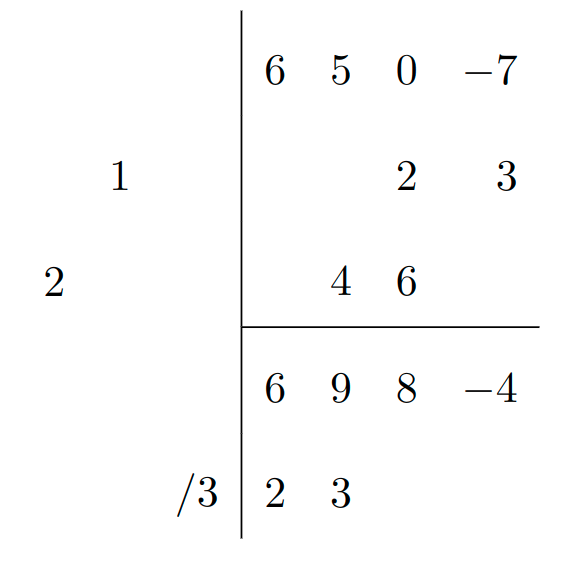
\includegraphics[width=0.4 \linewidth]{synthetic-division.png}
\end{center}



\end{document}
